% This is "sig-alternate.tex" V2.1 April 2013
% This file should be compiled with V2.5 of "sig-alternate.cls" May 2012
%
% This example file demonstrates the use of the 'sig-alternate.cls'
% V2.5 LaTeX2e document class file. It is for those submitting
% articles to ACM Conference Proceedings WHO DO NOT WISH TO
% Strictly ADHERE TO THE SIGS (PUBS-BOARD-ENDORSED) STYLE.
% The 'sig-alternate.cls' file will produce a similar-looking,
% albeit, 'tighter' paper resulting in, invariably, fewer pages.
%
% ----------------------------------------------------------------------------------------------------------------
% This .tex file (and associated .cls V2.5) produces:
%       1) The Permission Statement
%       2) The Conference (location) Info information
%       3) The Copyright Line with ACM data
%       4) NO page numbers
%
% as against the acm_proc_article-sp.cls file which
% does NOT produce 1) thru' 3) above.
%
% Using 'sig-alternate.cls' you have control, however, from within
% the source .tex file, over both the CopyrightYear
% (defaulted to 200X) and the ACM Copyright Data
% (defaulted to X-XXXXX-XX-X/XX/XX).
% e.g.
% \CopyrightYear{2007} will cause 2007 to appear in the copyright line.
% \crdata{0-12345-67-8/90/12} will cause 0-12345-67-8/90/12 to appear in the copyright line.
%
% ---------------------------------------------------------------------------------------------------------------
% This .tex source is an example which *does* use
% the .bib file (from which the .bbl file % is produced).
% TODO REMEMBER HOWEVER: After having produced the .bbl file,
% and prior to final submission, you *NEED* to 'insert'
% your .bbl file into your source .tex file so as to provide
% one 'self-contained' source file.
% ================= IF YOU HAVE QUESTIONS =======================
% Questions regarding the SIGS styles, SIGS policies and
% procedures, Conferences etc. should be sent to
% Adrienne Griscti (griscti@acm.org)
%
% Technical questions _only_ to
% Gerald Murray (murray@hq.acm.org)
% ===============================================================
%
% For tracking purposes - this is V2.0 - May 2012

\documentclass{sig-alternate-05-2015}
  \pdfpagewidth=8.5truein
  \pdfpageheight=11truein
  
  
% Custom package imports
\usepackage[utf8]{inputenc}
\usepackage{microtype}
\usepackage{booktabs}

\usepackage{graphicx}
\usepackage[utf8]{inputenc}
\usepackage{listings}
\usepackage{cleveref}
\usepackage{textcomp}
\usepackage[usenames, dvipsnames]{color}
\usepackage{url}

% Custom config
\graphicspath{{figures/}}

\definecolor{myviolett}{RGB}{127, 0, 85}
\definecolor{darkred}{RGB}{136, 0, 0}
\definecolor{darkblue}{RGB}{52, 89, 127}
\definecolor{lightgreen}{RGB}{44, 55, 0}

\lstset{
	basicstyle=\ttfamily\scriptsize,
	keywordstyle=\color{darkred}\ttfamily,
	stringstyle=\color{darkblue}\ttfamily,
	commentstyle=\color{lightgreen}\ttfamily,
	breaklines=true,
	aboveskip=.75\baselineskip,
	belowskip=1.5\baselineskip,
	upquote=true,
	showstringspaces=false
}

\lstdefinelanguage{dsl} % Farblich orientiert an Eclipse
{
	morekeywords={
		Feature,
		As,a,
		I, want, to,
		In, order, to,
		Scenario,
		Given, I, am, on, the, screen, 
		when, I, in, the, textfield, type, and,click,button,
		then, the, alert, is,
		Mapping, url,fragment,locator, label, nls, en, driver
	},
	sensitive=false, % keywords are not case-sensitive
	%morecomment=[l]{//}, % l is for line comment
	%morecomment=[s]{/*}{*/}, % s is for start and end delimiter
	morestring=[b]", % defines that strings are enclosed in double quotes
}

\lstdefinelanguage{xtext} % Farblich orientiert an Xtext Doku
{
	morekeywords={
		ID,	STRING, DOUBLE, MESSAGE,
		returns, current
	},
	sensitive=true, % keywords are case-sensitive
	%morecomment=[l]{//}, % l is for line comment
	%morecomment=[s]{/*}{*/}, % s is for start and end delimiter
	morestring=[b]', % defines that strings are enclosed in double quotes
	keywordstyle=\color{myviolett}\ttfamily,
	morekeywords={[2]{Person, UsualCase, Unknown, 
			ResultDeclaration, Query, 
			PlusOrMinus, MetricExpression, MulOrDiv, MetricAtomic, SumFunction, ColumnSelection, MetricsCountFunction, MetricsRef, DoubleConstant,
			RuleBody, RuleSpecification, WarnIf,
			Column, Requirement,
			Operator, RuleAtomic,
			Factor, MetricDefinition, Term,CountFunction, LengthFunction}},
	keywordstyle={[2]{\color{darkblue}}},
	stringstyle=\color{lightgreen}\ttfamily,
}

\crefname{lstlisting}{Listing}{Listings}
\crefname{figure}{Figure}{Figures}

\begin{document}

% Copyright
\setcopyright{acmcopyright}
%\setcopyright{acmlicensed}
%\setcopyright{rightsretained}
%\setcopyright{usgov}
%\setcopyright{usgovmixed}
%\setcopyright{cagov}
%\setcopyright{cagovmixed}


% the DOI
\doi{http://dx.doi.org/xx.xxxx/xxxxxxx.xxxxxxx}

% the ISBN
\isbn{978-1-4503-4486-9/17/04}

\acmPrice{\$15.00}

%
% --- Author Metadata here ---
\conferenceinfo{SAC'17,}{ April 3-7, 2017, Marrakesh, Morocco}
\CopyrightYear{2017} % Allows default copyright year (20XX) to be over-ridden - IF NEED BE.
%\crdata{0-12345-67-8/90/01}
% --- End of Author Metadata ---

\title{A Model-Driven Approach for Specification-Driven Automated UI Testing
%Possible alternative titles:
%A model driven approach for specifying automated UI tests
%A domain-specific language for defining automated UI tests
%Generating automated UI tests from formal requirement specifications
%Natural-language processing for test generation
%Automating UI tests from a scenario DSL
%\titlenote{(Produces the permission block, and copyright information). For use with SIG-ALTERNATE.CLS. Supported by ACM.}
}
%\subtitle{[Extended Abstract]
%\titlenote{A full version of this paper is available as \textit{Author's Guide to Preparing ACM SIG Proceedings Using \LaTeX$2_\epsilon$\ and BibTeX} at \texttt{www.acm.org/eaddress.htm}}}
%
% You need the command \numberofauthors to handle the 'placement
% and alignment' of the authors beneath the title.
%
% For aesthetic reasons, we recommend 'three authors at a time'
% i.e. three 'name/affiliation blocks' be placed beneath the title.
%
% You are NOT restricted in how many 'rows' of
% "name/affiliations" may appear. We just ask that you restrict
% the number of 'columns' to three.
%
% Because of the available 'opening page real-estate'
% we ask you to refrain from putting more than six authors
% (two rows with three columns) beneath the article title.
% More than six makes the first-page appear very cluttered indeed.
%
% Use the \alignauthor commands to handle the names
% and affiliations for an 'aesthetic maximum' of six authors.
% Add names, affiliations, addresses for
% the seventh etc. author(s) as the argument for the
% \additionalauthors command.
% These 'additional authors' will be output/set for you
% without further effort on your part as the last section in
% the body of your article BEFORE References or any Appendices.

\numberofauthors{1} %  in this sample file, there are a *total*
% of EIGHT authors. SIX appear on the 'first-page' (for formatting
% reasons) and the remaining two appear in the \additionalauthors section.
%
\author{
% You can go ahead and credit any number of authors here,
% e.g. one 'row of three' or two rows (consisting of one row of three
% and a second row of one, two or three).
%
% The command \alignauthor (no curly braces needed) should
% precede each author name, affiliation/snail-mail address and
% e-mail address. Additionally, tag each line of
% affiliation/address with \affaddr, and tag the
% e-mail address with \email.
%
% 1st. author
\alignauthor
%Christoph Rieger\\
%       \affaddr{ERCIS}\\
%       \affaddr{ERCIS, University of Münster}\\
       % TODO wirklich die Post-Adresse?
   %    \affaddr{Leonardo Campus 3}\\
   %    \affaddr{48149 Münster, Germany}\\
%       \affaddr{Münster, Germany}\\
%       \email{christoph.rieger@ercis.de}
- blinded for review -
}
%TODO weitere Autoren

% There's nothing stopping you putting the seventh, eighth, etc.
% author on the opening page (as the 'third row') but we ask,
% for aesthetic reasons that you place these 'additional authors'
% in the \additional authors block, viz.
%\additionalauthors{Additional authors: John Smith (The Th{\o}rv{\"a}ld Group, email: {\texttt{jsmith@affiliation.org}}) and Julius P.~Kumquat (The Kumquat Consortium, email: {\texttt{jpkumquat@consortium.net}}).}
\date{7 October 2016}
% Just remember to make sure that the TOTAL number of authors
% is the number that will appear on the first page PLUS the
% number that will appear in the \additionalauthors section.

\maketitle
\begin{abstract}
The most important key to success for a software project are concise and relevant requirements as recent research shows.
Requirement documents fulfilling these quality criteria include besides others an at least semi-formal description and an abstract UI description. 
However, stakeholder expectations change constantly during a project and requirement documents and especially UI descriptions are often not updated leading to severe problems in the development and testing phase.
This paper introduces an approach that automatically recognizes differences between requirement and UI descriptions and rewards up to date requirement documents.
The center of the approach is a domain-specific language that connects textual requirement descriptions to the corresponding abstract UI and thereby enables advanced validation and user support.
In addition to improving the overall quality of requirement documents, the language comes with a generator infrastructure to generate automated UI test cases for different UI frameworks such as Web and SWT. 
The focus of the approach is to ease the creation and validation of requirements documents incentivized by the automated UI test cases generated from the descriptions.
\end{abstract}

%
% The code below should be generated by the tool at
% http://dl.acm.org/ccs.cfm
% Please copy and paste the code instead of the example below. 
%
\begin{CCSXML}
	<ccs2012>
	<concept>
	<concept_id>10011007.10010940.10010971.10010980.10010984</concept_id>
	<concept_desc>Software and its engineering~Model-driven software engineering</concept_desc>
	<concept_significance>500</concept_significance>
	</concept>
	<concept>
	<concept_id>10011007.10011074.10011111.10011696</concept_id>
	<concept_desc>Software and its engineering~Maintaining software</concept_desc>
	<concept_significance>500</concept_significance>
	</concept>
	</ccs2012>
\end{CCSXML}

\ccsdesc[500]{Software and its engineering~Model-driven software engineering}
\ccsdesc[500]{Software and its engineering~Maintaining software}

%
%  Use this command to print the description
%
\printccsdesc

% We no longer use \terms command
%\terms{Theory}

\keywords{Domain-Specific Language, Behavior-Driven Development, Model-driven software development, Automated UI testing, Xtext}

\section{Introduction}
-	Well documented and up-to-date Requirements are crucial for project success
-	Many standards on how to describe requirements and what to include (functional, non-functional, UI-descriptions)
-	UI descriptions are an important part since they create a common ground for developers, testers and business analysts to discuss even before implementation has started
-	Because requirement documents play a central role in software development project every change affects multiple documents. If there is no traceability between the different artifacts it might happen that documents get not updated accordingly. Especially, in projects under time pressure documents will not be updated leading not only to outdated requirements but also to outdated documentation and more importantly outdated or irrelevant test cases.
-	The approach presented in this paper tries to encourage the requirements maintenance by rewarding it with fully generated automated test cases.
-	The domain specific language introduced combines wireframe UI descriptions with specification written in a ubiquitous language as defined by the behavior driven development process.
-	As for tools like cucumber the restriction applies: The main focus of the specification driven testing approach is to ensure a clean and up-to-date documentation of the system rewarded with fully generated test cases.
Well understood, documented and up-to-date requirements are crucial to successfully accomplishing a software development project.
There are many standards for software requirement such as [Quelle] and [Quelle] that all define the structure and the content of the textual requirement specifications and additional artifacts such as abstract UI description [Quelle for Standard].
Especially in projects following an agile process such as Scrum or Canban, requirements are documented by user stories encapsulating a specific function from a user’s perspective.
In addition, the Behavior Driven Development approach divides user stories in more detailed scenarios that come with a pre-defined format using an ubiquitous language to describe the expected behavior.


\section{Related Work}\label{sec:RelatedWork}
BDD Approach
Wireframing
Generating automated test cases


\section{Specification-Driven UI Tesing}\label{sec:SpecificationDrivenUITesting}
\subsection{Specifying the Application}\label{sec:SpecifyingTheApplication} 
The capabilities of the Specification Language are illustrated by creating wireframe, feature and mapping definitions for a simple calendar application.
The calendar web application consist of a login screen and an overview screen and is able to manage an users appointments. 
In the following a wireframesketcher model for the login screen and the overview screen are explained.
In addition, the feature file for the login screen is explained to illustrate some of the language capabilities to describe scenarios.
Finally, the mapping file is explained that contains rules to identify the widgets' implementation in the actual application.
All three files together are processed by a generator to create automated test cases.
\begin{figure}[h]
	\centering
	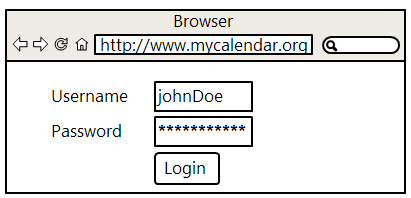
\includegraphics[width=0.8\linewidth]{Login.png}
	\caption{Wireframe sketch describing the Login screen.}
	\label{fig:login}
\end{figure}

\cref{fig:login} shows a wireframesketcher model of the login screen that has two text input fields and one button.
The graphical representation of the models are created using the wireframesketcher tool are backed by an Ecore model making it easy to integrate them with the domain-specific languages for feature and mapping definitions.
After entering a valid username and a valid password the login can be executed by clicking the login button leading to the overview screen as shown in \Cref{fig:overview}.
The expected behavior for the Login screen is described formally within a feature file that contains different scenarios.
\begin{lstlisting}[captionpos=b, caption=Feature Description: Login Screen., label={lst:featureLogin}, language=dsl]
Feature Login

As a "Calendar User"
I want to "login to the calendar application"
In order to "manage my appointments"

Scenario ValidLogin
Given I am on the screen Login 
when I type "johnDoe" in the Username textfield 
and I type "Password" in the Password textfield 
and I click the Login button
then I am on the the screen Overview 
and the Appointments table is visible
\end{lstlisting}

\Cref{lst:featureLogin} shows the feature description for the login screen that is divided into three main parts. 
The first part defines the feature name which in this case is \textit{Login}.
The name field is a crucial for references to this file as well as for later generation so that is restricted to alphabetical letters excluding special characters.

The second part explains the benefit of this feature from a customer perspective. 
The keyword sequences \textit{As a}, \textit{I want to}, and \textit{In order to} are predefined by the specification language grammar to ensure an uniform structure.
Although, the second part is optional and therefore not evaluated by the generators it is an important mechanism to verify the that a feature is really required (Quellen BDD).

The third part describes different scenarios for the same screen using a BDD like structure.
For a single screen there can be multiple scenarios within one feature file that describe different behavior, however, the sample shown above focuses on a successful login.
The \textit{Login} scenario starts with the context area in which the Login screen is set into context. 
Based on the screen in context the possible widgets, actions and their parameters are determined dynamically.
The following command area defines action executed on the screen.
The action introduced by the keyword sequence \textit{When I} is about typing the value ``\textit{johnDoe}" into the \textit{Username} textfield. 
While the \textit{When I} keyword sequences is proposed to structure the scenario description the keyword \textit{type} is proposed dependent on the widgets on the screen in context.
The second part of the When statement determines on which widget the action should be executed.
At this point only such widgets are considered valid that are on the screen and applicable for the action keyword.
Based on the underlying Ecore model, references can be validated at any time leading to early detection of test cases affected by renaming or removing of widgets.
Another When statement is attached using the \textit{and I} keyword sequence to type the password into the respective field.
The third command statement defines a click on the \textit{Login} button that causes an event in the application.
The expected response of the application to the event triggered by clicking the button, is described in the next part of the scenario description.

The last part of the scenario description is the assertion area in which the screen content is checked after the actions have been executed.
The first assertion changes the screen context of the scenario, since it is assumed that after a successful login the screen has changed.
In the example scenario from \cref{lst:featureLogin} it is assumed that the Overview screen is shown.
The following assertion statements introduced by \textit{and the} are now executed in the context of the \textit{Overview} screen which means that only widgets from that screen can be referenced.
\begin{figure}[h]
	\centering
	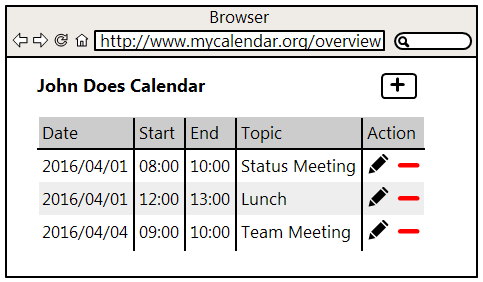
\includegraphics[width=0.8\linewidth]{Overview.png}
	\caption{Wireframe sketch describing the Overview screen.}
	\label{fig:overview}
\end{figure}

\Cref{fig:overview} Shows the Overview screen that is shown after a successful login and contains a table showing all known appointments and a plus button to add new entries.
To describe further scenarios for this screen a separate feature file is created.
To generate automated test cases from the screen and feature specification a mapping is required that maps the logical elements on the screen to their implementation.

\begin{lstlisting}[captionpos=b, caption=Mapping Description: Login Screen., label={lst:mappinglogin}, language=dsl]
Mapping Login

url {fragment:"#/login"}
label {nls{en:"Login"}}
Username{
	locator:"#username"
}
Password{
	locator:"#password"
}
Login{ 
    driver: org.sample.calendar.ButtonDriver
    locator:"#login"
}
\end{lstlisting}

\Cref{lst:mappinglogin} shows the mapping description for the Login screen.
The first part of the file states the URL part needed to find the screen within the application which is ``\#/login". 
After the keyword \textit{label} the label of the page as shown in the browser is stated, which can be used for identifying and verifying the correct screen within the application.

The second part of the mapping files contains one entry for each widget on the screen.
As in the feature file, \textit{Username},\textit{Password}, and \textit{Login} are real references to the elements from the wireframesketcher Ecore model.
Since these can be validated feedback on the impact of changing a widget's or screen's name on the mapping files can be given early.
For every widget there is one \textit{locator} which in case of a web application could be the ID of the element in the HTML document tree (Reference to HTML DOM).
For custom widgets or such that cannot be found using a simple ID mechanism a custom driver can be specified as shown for the \textit{Login} button.
Explicitly stating a \textit{driver} will make the automated test try to reach out to the widget using the custom driver. 
The mechanism enables the use of custom widgets without applying any changes to the screen or feature files.

The combination of screen, feature, and mapping file is used by the a generator to create a page object and a test script.
The first, encapsulates all interactions, such as clicking, typing, resolving a label, per screen in a single object.
Basis for the page objects is the combination of screen and mapping files.
For the example shown in \Cref{lst:featureLogin} there are two mapping files needed one for the \textit{Login} and one for the \textit{Overview} screen.

The second generation results are the test scripts that are generated by using the information from the screen and feature files.
Every scenario is turned into a test method containing all actions and assertions from the feature file.
After being generated the test cases can be executed locally within Eclipse or in a maven build on a continuous integration environment.


\subsection{Composition of the Specification Language}
\subsubsection{Specification Language Architecture}
Figure to show how everything interacts
\subsubsection{Wireframesketcher Integration}
Existing Framework used to specify wireframes within an eclipse environment.
EMF Based to easily integrate with the Xtext based DSLs.
Metamodel patched to add some marker interfaces
Metamodel general structure
Xtext Adapter added to make model elements referable from the outside.

\subsubsection{Feature DSL}
Feature DSL defines the structure of a feature file as well as re-usable language parts
Based on the Control Action Parameter from Jubula.
Possible sentences are always based on the current scope
Advanced concepts (parameter, depends on)
Execution sequence as stated

\subsubsection{Mapping DSL DSL}
Maps logical elements from the screen to real world implementations
Driver concept
Identify by ID
Validations


\subsubsection{Generator}
Takes feature and mapping file in combination with the wireframesketch to generate test cases
The generator infrastructure allows different generator for different UI Frameworks. In the default implementation there is a generator for Web applications
In addition, there have been proprietary generators for SWT based RCP applications
The generators can currently be configured per Eclipse workspace.
Generator generates Cucumber specifications files that are able to run web-based test with spock as execution framework and selenium as web driver underneath. 
The logic to access the elements on each page is encapsulated in page objects (fowler) that are also generated from the screen files. Some of the functionality generated into the page objects relies on library methods that come with the framework. 
The generator can be integrated in a CI environment like Jenkins. In such an environment it will take the feature, mapping and screen files and turn them into Cucumber specification, before they are executed. 

\section{Discussion}\label{sec:Discussion}
Not introducing a new tool or technique, but bringing existing approaches together

\section{Conclusion}\label{sec:Conclusion} %and Future Work
Especially after the first release of a functionality the user stories and UI description become less relevant, because discussion now focusses on the running application. Mitigate this by putting the feature description and the UI description in the focus of development 
Not only generate Testcases, but also generate implementation, especially in the UI area.
Web-enable to increase non-technical user’s acceptance. 
Focus on Service tests in the same way (replay UI description by formal Service Descriptions such as WSDL)
Improve process inclusion (write scenarios in HP Quality Center and report execution back to HP QC). 
Language Design Currently little bit technical to ease scoping could be changed. Leading to advanced scoping and content assist mechanisms to achieve 


%\newpage
%
% The following two commands are all you need in the
% initial runs of your .tex file to
% produce the bibliography for the citations in your paper.
%IMPORTANT directly embedded
\bibliographystyle{abbrv}
\bibliography{specification_driven_testing}  % sigproc.bib is the name of the Bibliography in this case

%\begin{thebibliography}{10}
%\end{thebibliography}

% You must have a proper ".bib" file
%  and remember to run:
% latex bibtex latex latex
% to resolve all references
%
% the ACM needs 'a single self-contained file'!
%
%\balancecolumns
\begin{comment}
\appendix
%Appendix A
\section{Headings in Appendices}
\subsection{References}
Generated by bibtex from your ~.bib file.  Run latex,
then bibtex, then latex twice (to resolve references)
to create the ~.bbl file.  Insert that ~.bbl file into
the .tex source file and comment out
the command \texttt{{\char'134}thebibliography}.
%\balancecolumns
\end{comment}
\end{document}
